%! Author = Wiktor Rostkowski
%! Date = 28/05/2024
\newgeometry{} % Ustawienie mniejszych marginesów górnych i dolnych

\chapter{Analiza wymagań}
\label{ch:analiza-wymagan}

\section{Sposób gromadzenia wymagań}
\label{sec:sposob-gromadzenia-wymagan}

Wymagania dla projektu zostały wybrane przez zespół projektowy~w~pierwszym semestrze. Zostały określone na podstawie analizy aktualnych rozwiązań oraz potrzeb zespołu projektowego.

Na podstawie opracowanego dokumentu \glslink{sws}{SWS}, przygotowano wymagania dotyczące funkcjonalności projektu. \newline Wykorzystana została metodyka priorytezacji wymagań \glslink{moscow}{MoSCoW}\footnote{Metoda MoSCoW – Must, Should, Could, Won't}[]:
\begin{itemize}
    \item \textbf{M – must (musi być)} – wymaganie bezkompromisowo musi zostać zrealizowane, bez niego projekt nie zostanie ukończony;
    \item \textbf{S – should (powinno być)} – wymaganie powinno być zrealizowane, jeżeli tylko jest taka możliwość;
    \item \textbf{C – could (może być)} – wymaganie powinno być zawarte~w~projekcie, jeśli wystarczy~na~nie czasu;
    \item \textbf{W – won't (nie będzie)} – wymaganie nie powinno być zawarte~w~tym wydaniu projektu, ale może być zrealizowane~w~przyszłości.
\end{itemize}


\section{Udziałowcy}
\label{sec:udzialowcy}

\begin{stakeholder}[label={tab:stakeholder:someholder1},caption={opis udzialowca}]
    \id{UOB1}
    \name{Podstawowy użytkownik aplikacji (np. Turysta) }
    \descr{Osoba korzystająca z aplikacji~w~celu poznawania \glslink{poidef}{POI} i optymalnego przemieszczania się między nimi }
    \type{Ożywiony bezpośredni}
    \viewpoint{Użytkownik  operator}
    \limitations{Wymaga umiarkowanych umiejętności technicznych}
    \requ{F01,WO6,WO7, FO1, FO2, FO3, FO5, FO7, FO8, FO9, FO10, FO11, FO12, FO13, FO14, FO15, FO17, FO18, FO21, FO22, FO23, FO24, FO26, IO1, IO2, IO3, IO5, IO6, NFO1, ŚDO2}
\end{stakeholder}

\begin{stakeholder}[label={tab:stakeholder:someholder2},caption={Opis udzialowca}]
    \id{UOB2}
    \name{Zespół projektowy}
    \descr{Pomysłodawcy i autorzy rozwiązania}
    \type{Ożywiony bezpośredni}
    \viewpoint{Techniczny}
    \limitations{Ograniczony czas realizacji projektu}
    \requ{WO1, WO2, WO3, WO4, WO5, WO6, WO7, FO1, FO2, FO3, FO4, FO5, FO7, FO8, FO9, FO10, FO11, FO12, FO13, 
    FO14, FO15, FO16, FO18, FO19, FO20, FO21, FO22, FO23, FO24, FO25, IO1, IO2, IO3, IO4, IO5, IO7, NFO1, NFO2, ŚDO1, ŚDO2}
\end{stakeholder}

\begin{stakeholder}[label={tab:stakeholder:someholder3},caption={Opis udzialowca}]
    \id{UOB3}
    \name{Firmy o charakterze najmu krótko-terminowym }
    \descr{Firmy o charakterze najmu krótko-terminowego mające bezpośredni kontakt z turystami}
    \type{Ożywiony niebezpośredni }
    \viewpoint{Współpraca z turystami}
    \limitations{Brak}
    \requ{WO7, FO3, FO5, FO9, FO21, FO22, FO24, IO1, IO2, IO3, ŚDO2}
\end{stakeholder}

\section{Wymagania ogólne i dziedzinowe}
\label{sec:wymagania-ogolne-i-dziedzinowe}


\begin{requirementstab}[label={tab:requirements:general1},caption={Karta wymagania: Obsługa użytkowników}]
    \id{WO1}
    \priority{M}
    \name{Obsługa użytkowników}
    \descr{System obsługuje użytkowników zalogowany, jak i niezalogowanych do systemu }
    \sholder{UOB2}
    \reqrelated{WO9, F24,}
\end{requirementstab}
\begin{requirementstab}[label={tab:requirements:general2},caption={Karta wymagania: Działanie~w~czasie rzeczywistym Offline}]
    \id{WO2}
    \priority{C}
    \name{Działanie~w~czasie rzeczywistym offline lub online }
    \descr{Aplikacja musi działać i synchronizować dane do 15 minut. 
    Wersja offline wykorzystuje ostatnie zapisane informacje takie jak podgląd wcześniej zaplanowanych wycieczek}
    \sholder{UOB2}
\end{requirementstab}
\begin{requirementstab}[label={tab:requirements:general3},caption={Karta wymagania: Panel administracyjny}]
    \id{WO3}
    \priority{S}
    \name{Zarządzanie danymi z poziomu aplikacji}
    \descr{Możliwość sprawdzanie aktualnych danych \glslink{poidef}{POI} poprzez panel aplikacji internetowej (Panel administracyjny) }
    \sholder{UOB2}
    \reqrelated{FO4, IO7}
\end{requirementstab}
\begin{requirementstab}[label={tab:requirements:general4},caption={Karta wymagania: Licencje i prawa}]
    \id{WO4}
    \priority{M}
    \name{Licencje i prawa}
    \descr{Wszystkie technologie, narzędzia, wzorce oraz inne elementy niezbędne do realizacji systemu muszą być licencjonowane i pochodzić bezpośrednio od głównych dostawców, a nie od pośredników. }
    \sholder{UOB2}
    \reqrelated{Wszystkie}
\end{requirementstab}
\begin{requirementstab}[label={tab:requirements:general5},caption={Karta wymagania: Responsywny interfejs}]
    \id{WO5}
    \priority{M}
    \name{Responsywny interfejs}
    \descr{Interfejs użytkownika powinien być wykonany zgodnie z praktyką programowania responsywnych stron internetowych.  }
    \sholder{UOB2}
    \reqrelated{NFO2,ŚO2}
\end{requirementstab}
\begin{requirementstab}[label={tab:requirements:general6},caption={Karta wymagania: Rejestracja użytkowników}]
    \id{WO6}
    \priority{S}
    \name{Rejestracja użytkowników  }
    \descr{Rejestracja powinna przebiegać sprawnie, zgodnie ze wszystkimi standardami i przepisami prawa, a przede wszystkim musi być zgodna z RODO.  }
    \sholder{UOB2, UOB1}
    \reqrelated{WO1}
\end{requirementstab}
\begin{requirementstab}[label={tab:requirements:general7},caption={Karta wymagania: Komercjalizacja}]
    \id{WO7}
    \priority{S}
    \name{Komercjalizacja }
    \descr{Aplikacja ma umożliwiać reklamowanie swoich usług partnerom biznesowym~w~sposób spójny z interfejsem.  }
    \sholder{UOB1, UOB2, UOB3}
    \reqrelated{FO1, IO5, IO6 }
\end{requirementstab}

\section{Wymagania funkcjonalne}
\label{sec:wymagania-funkcjonalne}

\begin{requirementstab}[label={tab:requirements:func1},caption={Karta wymagania: Interaktywna mapa}]
    \id{FO1}
    \priority{M}
    \name{Interaktywna mapa}
    \descr{Jako turysta chciałbym, zobaczyć mapę wszystkich atrakcji dostępnych~w~mieście z lotu ptaka 
    }
    \acceptcrit{Użytkownik może zobaczyć aktualne dostępne atrakcje dostępne~w~danym mieście }
    \inputdata{Użytkownik, włączając aplikacje widzi przedstawioną mapę}
    \preconditions{ Dostępność systemów partnerów, głównie \glslink{stadiamaps}{Stadia Maps}   }
    \postconditions{ Wyświetlenie atrakcji. }
    \exceptions{ Wyświetlanie komunikatu~w~przypadku niedostępności atrakcji~w~aktualnej chwili oraz przedstawienia propozycji zmiany punktu docelowego. }
    \implementation{ Użytkownik, korzystając z przeglądarki lub aplikacji, widzi interaktywną mapę z atrakcjami~w~danym mieście.}
    \sholder{UOB1, UOB2 }
    \reqrelated{FO5, IO3,IO4}
\end{requirementstab}
\begin{requirementstab}[label={tab:requirements:func2},caption={Karta wymagania: Dane czasu rzeczywistego }]
    \id{FO2}
    \priority{S}
    \name{Wyświetlanie powiadomień o zmianach. }
    \descr{\begin{itemize}
        \item Jako Turysta 
        \item chcę dostawać powiadomienia o zmianach~w~planie,
        \item bo wtedy nie spóźnię się na czas otwarcia atrakcji. 
    \end{itemize}
    }
    \acceptcrit{Powiadomienie będzie, zgodnie z aktualnym planem  }
    \inputdata{Aplikacja pamięta, jakie użytkownik wybrał atrakcje do odwiedzenia i informuje o zmianach po synchronizacji. }
    \preconditions{ Użytkownik  odwiedził stronę i posiada zapisane atrakcje.  }
    \postconditions{ Aplikacja przedstawi nowe zmiany po kliknięciu powiadomienie.   }
    \exceptions{ Użytkownik nie zezwolił powiadomienia bądź nowe dane nie istnieją. }
    \implementation{ Na planie zajęć wyświetlają się nowe zmiany~w~innym kolorze  }
    \sholder{UOB1, UOB2 }
\end{requirementstab}
\begin{requirementstab}[label={tab:requirements:func3},caption={Karta wymagania: Widok listy \glslink{poidef}{POI}}]
    \id{FO3}
    \priority{M}
    \name{Zakładka z przestawionymi dostępnymi wszystkimi atrakcjami  }
    \descr{\begin{itemize}
        \item Jako użytkownik  
        \item chce korzystać z aplikacji z listą dostępnych atrakcji~w~wersji tekstowej,
        \item ponieważ chce zobaczyć dostępne spektrum możliwości, bez szukania informacji na mapie i przeciągania. 
    \end{itemize}
    }
    \acceptcrit{Lista dostępnych \glslink{poidef}{POI}. }
    \inputdata{Brak}
    \preconditions{ Użytkownik wszedł na stronę z dostępnymi atrakcjami.  }
    \postconditions{ Użytkownik może przeczytać lub klikać na interesujące go atrakcje.   }
    \exceptions{ Brak dostępnych atrakcji~w~wyznaczonym zakresie czasowym  }
    \implementation{ Widok listy daje możliwość dodanie atrakcji do koszyka oraz przedstawia opis POI}
    \sholder{UOB1, UOB2, UOB3 }
    \reqrelated{FO5}
\end{requirementstab}
\begin{requirementstab}[label={tab:requirements:func4},caption={Karta wymagania: Panel zarządzania atrakcjami}]
    \id{FO4}
    \priority{M}
    \name{Panel zarządzania atrakcjami. }
    \descr{\begin{itemize}
        \item Jako administrator 
        \item potrzebuję panelu do zarządzania danymi atrakcji turystycznych wspomaganego sztuczną inteligencją,
        \item aby szybko reagować na zmiany wprowadzane przez właścicieli atrakcji turystycznych. 
    \end{itemize}
    }
    \acceptcrit{Lista dostępnych punktów. }
    \inputdata{Konto z uprawnieniami administracyjnymi}
    \preconditions{ Użytkownik wszedł na ukrytą stronę z panelem.  }
    \postconditions{ Można wykonywać podstawowe operacje \glslink{CRUD}{CRUD}   }
    \exceptions{ Jest możliwość dodawania kolejnych atrakcji. Sztuczna inteligencja może błędnie wykonać swoje zadanie.   }
    \implementation{ Panel administracyjny do zarządzania wszystkimi elementami składowymi POI zdjecia, nazwa, opis, link do strony z opisem.   }
    \sholder{ UOB2 }
    \reqrelated{W03,FO5,IO7}
\end{requirementstab}
\begin{requirementstab}[label={tab:requirements:func5},caption={Karta wymagania: Punkty interaktywnej mapy}]
    \id{FO5}
    \priority{M}
    \name{Znaczniki na interaktywnej mapie informujące o \glslink{poidef}{POI}.}
    \descr{Jako użytkownik chce móc wyświetlić wybrane atrakcje, które mnie interesują,
         ponieważ  umożliwi to spojrzenie na opis \glslink{poidef}{POI}.
    
    }
    \acceptcrit{Mapa posiada znaczniki atrakcji dodanych poprzez administratora. Po kliknięciu znacznika pojawią się szczegółowe informacje o \glslink{poidef}{POI} }
    \inputdata{Otwiera Aplikacje. }
    \preconditions{ Mapa Atrakcji ze znacznikami dodanymi przez administratora  aplikacji.}
    \postconditions{Brak}
    \exceptions{Brak dostępności API, aplikacja powinna wtedy pokazać błąd i próbować pobrać dane ponownie    }
    \implementation{ Mają być duże znaczniki ze zdjęciami atrakcji, które po kliknięciu otwierają szczegółowy widok    }
    \sholder{ UOB1, UOB2, UOB3  }
    \reqrelated{F01}
\end{requirementstab}
\begin{requirementstab}[label={tab:requirements:func6},caption={Karta wymagania: Oceny użytkowników }]
    \id{FO6}
    \priority{C}
    \name{Oceny użytkowników}
    \descr{Jako użytkownik chce mieć możliwość oceniania atrakcjami gwiazdkami~w~skali od jeden do pięciu,
         ponieważ chciałbym podzielić się swoją opinią.

    }
    \acceptcrit{Każda atrakcja ma możliwość dodawania opinii. }
    \inputdata{Posiadanie konta Opinia~w~skali od jeden do pięciu }
    \preconditions{ Można dodawać opinię liczbową.}
    \postconditions{ Brak  }
    \exceptions{ Użytkownik nie posiada konta albo został zablokowany na platformie.   }
    \implementation{ Przy danym punkcie zainteresowania (\glslink{poidef}{POI}) dostępny jest przycisk z opcją dodania opinii, a powyżej wyświetlana jest średnia ocen. Każdy użytkownik może dodać jedną opinię~w~formie gwiazdek od 1 do 5.    }
    \sholder{ UOB1  }
    \reqrelated{FO5,F07}
\end{requirementstab}
\begin{requirementstab}[label={tab:requirements:func7},caption={Karta wymagania: Zdjęcia użytkowników + tekst}]
    \id{FO7}
    \priority{C}
    \name{Możliwość pisania opinii wraz ze zdjęciami pod punktami zainteresowania.}
    \descr{Jako użytkownik chce możliwość pisania pisemnych opinii z możliwością dodania zdjęcia,
         aby móc przekazać większy kontekst moich opinii. 
    
    }
    \acceptcrit{Opinia musi zostać zatwierdzona przez administratora, można dodać na późniejszym etapie na podstawie algorytmu, który spełnia jakąś politykę prywatności. }
    \inputdata{Posiadanie konta zdjęcia, tekst }
    \preconditions{ Można dodawać opinie (ewentualnie ze zdjęciem).}
    \exceptions{Brak konta, za duże zdjęcie, nieprawidłowy format zdjęcia      }
    \implementation{ Przy danym \glslink{poidef}{POI} po kliknięciu, jest dostępny przycisk z opcją napisania opinia, każdy użytkownik może dodać jedną opinię.
    Opinia musi zostać zatwierdzona przez moderatora, nowe opinie wyświetlają się~w~panelu administratora.  Formularz dodawania zdjęcia używa kompresji formatu zdjęcia. }
    \sholder{ UOB1  }
    \reqrelated{FO5, F06,FO25}
\end{requirementstab}
\begin{requirementstab}[label={tab:requirements:func8},caption={Karta wymagania: Zapisane atrakcje turystyczne}]
    \id{FO8}
    \priority{S}
    \name{Zapisywanie list wybranych \glslink{poidef}{POI} pod konkretną nazwą.}
    \descr{Jako użytkownik chce możliwość zapisania wybranej trasy,
         ponieważ umożliwi to przygotowanie trasy na później. 
    
    }
    \acceptcrit{ Po wybraniu trasy, która zostanie przedstawiona, wyskakuje dymek z zapytaniem, czy  chcesz dodać tę trasę do ulubionych}
    \preconditions{ Zaplanowanie trasy~w~poprzednich widokach aplikacji }
    \postconditions{  Brak }
    \exceptions{ Jeśli użytkownik jest offline lub niezalogowany, pojawia się komunikat o błędzie:
     "Aby dodać trasę, należy być zalogowanym i mieć połączenie z internetem."   }
    \implementation{ Możliwość otworzenia zapisanej, optymalnej trasy bez konieczności ponownego jej obliczania oraz bez połączenia internetowego.}
    \sholder{ UOB1, UOB2 }
    \reqrelated{F09,FO26}
\end{requirementstab}

\begin{requirementstab}[label={tab:requirements:func9},caption={Karta wymagania: Udostępnianie zapisanych list \glslink{poidef}{POI}}]
    \id{FO9}
    \priority{C}
    \name{Udostępnianie zapisanych list \glslink{poidef}{POI} pomiędzy użytkownikami}
    \descr{Jako użytkownik chce mieć możliwość udostępnienia wybranej trasy,
         ponieważ umożliwi to polecania wybranych trasy. 
    
        }
    \acceptcrit{ W zakładce zapisanych listy widniej dymek z udostępnię danej trasy}
    \inputdata{Użytkownik klika  przycisk udostępnienia trasy.  }
    \preconditions{ Posiadanie zapisanej trasy  }
    \postconditions{     Użytkownik udostępniający musi przekazać link do udostępnionej trasy, 
     użytkownik otrzymujący link musi zaakceptować udostępnioną trasę  }
    \exceptions{  Nie można przekroczyć 100 zapisanych tras.  }
    \implementation{ Każda trasa ma indywidualny kod~w~bazie danych. Właściciel trasy może ją edytować. a zobaczyć może każda osoba posiadająca link.}
    \sholder{ UOB1, UOB2, UOB3   }
    \reqrelated{F08,FO26}
\end{requirementstab}
\begin{requirementstab}[label={tab:requirements:func10},caption={Karta wymagania: Wyznaczanie trasy pieszej }]
    \id{FO10}
    \priority{M}
    \name{Wyznaczanie optymalnej trasy pieszej pomiędzy wybranymi \glslink{poidef}{POI}}
    \descr{Jako użytkownik chcę~w~sposób automatyczny wyznaczyć optymalną trasę między atrakcjami, aby wiedzieć, jak map się przedostać do danej atrakcji
    }
    \acceptcrit{ Algorytm wyznacza trasę od wybranego punktu pomiędzy 2 podanymi punktami na mapie.}
    \inputdata{Wybrane 2 atrakcje turystyczne - trasę.  }
    \preconditions{ Brak }
    \postconditions{ Brak  }
    \exceptions{ Brak dostępnej trasy między podanymi punktami  }
    \implementation{ Implementacja na podstawie przeszukiwania wszerz i kolejki priorytyzacji.    }
    \sholder{ UOB1, UOB2   }
    \reqrelated{F09}
\end{requirementstab}
\begin{requirementstab}[label={tab:requirements:func11},caption={Karta wymagania: Wyznaczanie optymalnej trasy z udziałem komunikacji miejskiej}]
    \id{FO11}
    \priority{S}
    \name{Wyznaczanie optymalnej trasy z udziałem komunikacji miejskiej}
    \descr{Jako użytkownik chce mieć możliwość przejścia wybranej trasy pieszo oraz dostępnej komunikacji miejskiej,
         aby przyśpieszyć podróż i zaoszczędzić czas
    }
    \acceptcrit{ Możliwość wyboru trasy z udziałem komunikacji miejskiej.}
    \inputdata{Wybrane 2 \glslink{poidef}{POI} }
    \preconditions{ Przedstawienie trasy podstawie wybranych punktów. }
    \postconditions{ Brak albo połączenie z internetem, aby aktualizować na bieżąco rozkład jazdy  }
    \exceptions{ Zaproponowanie innego transportu np. pieszo  }
    \implementation{ Dodanie integracji z API komunikacji miejskiej, synchronizując dane aktualnych rozkładów jazdy do proponowanej trasy.}
    \sholder{ UOB1, UOB2   }
    \reqrelated{F09,FO10}
\end{requirementstab}
\begin{requirementstab}[label={tab:requirements:func12},caption={Karta wymagania: Wyznacznia optymalnej trasy z udziałem samochodów osobowych}]
    \id{FO12}
    \priority{S}
    \name{Wyznaczanie optymalnej trasy z udziałem samochodów osobowych}
    \descr{Jako użytkownik chce mieć możliwość odbyć wybraną trase z udziałem samochodu,
         ponieważ umożliwi to wykorzystanie szybszego transportu z punktu A do B. 
    }
    \acceptcrit{ Algorytm umożliwia planowanie trasy z użyciem dróg przeznaczonych dla samochodów przy zachowaniu przepisów prawa drogowego takich jak drogi jednokierunkowe}
    \inputdata{Wybrane 2 \glslink{poidef}{POI} }
    \preconditions{ Brak}
    \postconditions{  Algorytm zaprezentował  trasę z wykorzystaniem dróg przeznaczonych dla samochodów     }
    \exceptions{ Brak trasy możliwej do pokonania samochodem     }
    \implementation{ Dodanie planowania trasy na podstawie dróg dostępnych tylko dla pojazdów do trzy i pół tony, używając OpenStreetMap   }
    \sholder{ UOB1, UOB2   }
    \reqrelated{IO1,F09,FO10,FO11}
\end{requirementstab}
\begin{requirementstab}[label={tab:requirements:func13},caption={Karta wymagania: Podgląd Wygenerowanej optymalnej trasy }]
    \id{FO13}
    \priority{M}
    \name{Widok wygenerowanej optymalnej trasy z możliwością podglądu jej na osi czasu}
    \descr{Jako użytkownik chce mieć możliwość przejrzenia całej trasy,
         ponieważ umożliwi to przejrzenia zaproponowanej trasy, atrakcja po atrakcji. 
    
    }
    \acceptcrit{ Widok listy zawierającej wszystkie uprzednio wybrane atrakcje turystyczne wraz z podstawowymi informacjami o nich oraz trasy pomiędzy nimi.}
    \inputdata{ Uprzednio wygenerowany plan zwiedzania}
    \preconditions{ Brak }
    \postconditions{ Dostęp do internetu, aby pobrać aktualizacje trasy~w~przypadku zmian danych. }
    \exceptions{  Brak wybranego planu zwiedzania }
    \implementation{ Z lewej strony widać proponowaną trasę a z prawej strony ekranu widać oś czas z wybranymi atrakcjami. Użytkownik może modyfikować trasę oraz wybierać konkretne punkty na trasie, 
   ~w~celu bliższego przyjrzenia się nim}
    \sholder{ UOB1, UOB2, UOB3   }
    \reqrelated{F09,FO10,FO11,FO12,FO14, FO15, FO16,F27}
\end{requirementstab}
\begin{requirementstab}[label={tab:requirements:func14},caption={Karta wymagania: Widok kalendarza podróży }]
    \id{FO14}
    \priority{M}
    \name{Widok kalendarza podróży trasy powinien umożliwiać zmianę kolejności odwiedzania na osi czasu \glslink{poidef}{POI} co~w~efekcie dostosuje resztę optymalnej trasy}
    \descr{Jako użytkownik chce mieć możliwość ustalania godzin zwiedzania,
         ponieważ kalendarz pokaże mi możliwość edycji trasy wycieczki optymalnej do godzin otwarcia. 
    
    }
    \acceptcrit{ Użytkownik może wybrać każdy element z proponowanej trasy i go zmienić}
    \inputdata{Wybrane atrakcje turystyczne – trasa np. Zapisana trasa lub stworzenie nowej trasy.  }
    \preconditions{ Zedytowana nowa trasa. }
    \postconditions{ Prezentacja nowej trasy o nowe sugestie~w~podróży.  }
    \exceptions{  Brak przeładowania trasy przez brak internetu. }
    \implementation{ Poprzez przesuwanie punktów na osi czasu jest możliwość manipulowania trasą.}
    \sholder{ UOB1, UOB2 }
    \reqrelated{F09,FO10,FO11,FO12,FO14, FO15}
\end{requirementstab}
\begin{requirementstab}[label={tab:requirements:func15},caption={Karta wymagania: \glslink{poidef}{POI} użytkowników }]
    \id{FO15}
    \priority{C}
    \name{Użytkownicy powinni mieć możliwość dodawania na mapę własnych \glslink{poidef}{POI}}
    \descr{Jako użytkownik chce mieć możliwość dodania nowych punktów i usunięcia z aktualnej listy dostępnych punków,
         ponieważ chciałbym wyznaczyć trasę między punktami, którymi administratorzy nie dodali. 
    
    }
    \acceptcrit{ Możliwość dodania niestandardowego punktu startowego i końcowego.}
    \inputdata{ Zalogowany użytkownik}
    \preconditions{ Brak }
    \postconditions{ Baza punktów użytkownika posiada nowo zapisany punkt }
    \exceptions{  Brak punktów niestandardowych lub punkt nie mieści się~w~obrębie dostępnej mapy. }
    \implementation{ Na interaktywnej mapie powinien znajdować się przycisk do dodania własnych atrakcji, ale tylko, gdy użytkownik jest zalogowany.}
    \sholder{ UOB1, UOB2   }
    \reqrelated{F09,FO10,FO11,FO12,FO14, FO15}
\end{requirementstab}
\begin{requirementstab}[label={tab:requirements:func16},caption={Karta wymagania: Środek transportu rower}]
    \id{FO16}
    \priority{C}
    \name{Wybór środka transportu rower}
    \descr{Jako użytkownik chce możliwość  wyznaczenia trasy z wykorzystanie roweru np. \glslink{mevo}{mevo}, 
         ponieważ chciałbym korzystać ze swojego roweru bądź wypożyczonego podczas zwiedzania. 
    
    }
    \acceptcrit{ Aplikacja ma tryb trasy rowerej}
    \inputdata{Wybrane atrakcje turystyczne }
    \preconditions{Przestawia optymalną trasę   }
    \postconditions{ Trasa zostaje przedstawiona użytkownikowi. }
    \exceptions{ Brak atrakcji brak planu.}
    \implementation{ Algorytm optymalnej trasy powinien brać pod uwagę czas potrzeby na zwiedzenie konkretnej atrakcji.
    Algorytm optymalnej trasy powinien brać pod uwagę czas przeznaczony na zwiedzenia~w~ciągu danego dnia.
    Algorytm optymalnej trasy powinien brać pod uwagę dni przeznaczone na zwiedzanie.
    Algorytm optymalnej trasy powinien brać pod uwagę status atrakcji (np otwarte tylko~w~środy o konkretnych godzinach).
    Algorytm optymalnej trasy powinien brać pod uwagę warunki pogodowe i przesuwać \glslink{poidef}{POI} wymagające odpowiedniej kolejności względem siebie, jeśli to możliwe.
    Algorytm optymalnej trasy powinien informować użytkownika o zmianie pogody i powinien zaproponować alternatywny plan zwiedzania.}
    \sholder{ UOB2 }
    \reqrelated{FO20}
\end{requirementstab}
\begin{requirementstab}[label={tab:requirements:func17},caption={Karta wymagania:  Aktualna pozycja użytkownika na interaktywnej mapie}]
    \id{FO17}
    \priority{C}
    \name{Aktualna pozycja użytkownika na interaktywnej mapie}
    \descr{Jako użytkownik chce widzieć swoją pozycję na mapie, 
         aby móc ocenić postępy~w~trasie.
    
    } 
    \acceptcrit{ Pozycja użytkownika (gps) }
    \inputdata{Wybrane atrakcje turystyczne – inicjacja trasy. }
    \preconditions{Zgoda użytkownika na dostęp do lokalizacji}
    \postconditions{ Brak }
    \exceptions{  Brak zgody użytkownika na dostęp do lokalizacji lub zgubiony sygnał GPS }
    \implementation{ Aplikacja na podstawie danych GPS pokazuje postęp użytkownika.}
    \sholder{ UOB1 }
    \reqrelated{FO17}
\end{requirementstab}
\begin{requirementstab}[label={tab:requirements:func18},caption={Karta wymagania: Filtracja \glslink{poidef}{POI} }]
    \id{FO18}
    \priority{C}
    \name{Filtracja atrakcji turystycznych}
    \descr{Jako użytkownik chce możliwość filtrowanie atrakcji po kategoriach takie jak ilość osób czy nazwa,
         ponieważ chciałbym mieć dokładniejszej selekcji \glslink{poidef}{POI}.
    
    }
    \acceptcrit{ Możliwości wyboru kategorii \glslink{poidef}{POI}}
    \inputdata{Wybrana kategoria. }
    \preconditions{     Włączony widok interaktywnej mapy lub listy \glslink{poidef}{POI}}
    \postconditions{ Brak }
    \exceptions{ Brak }
    \implementation{ Możliwość filtrowania \glslink{poidef}{POI} na podstawie wyznaczonych kategorii. Rozpisać na 2 widoki: listę i mapę, gdzie to ma się znajdować.
    }
    \sholder{UOB1, UOB2 }
    \reqrelated{FO5,FO20,FO21,}
\end{requirementstab}
\begin{requirementstab}[label={tab:requirements:func19},caption={Karta wymagania: Widok wybranych atrakcji}]
    \id{FO19}
    \priority{S}
    \name{Koszyk POI}
    \descr{Widok koszyka atrakcji przedstawiający wszystkie dodane \glslink{poidef}{POI} jakimi zainteresowany jest użytkownik do zwiedzenia.
    }
    \acceptcrit{ koszyk przechowuje dodane \glslink{poidef}{POI} }
    \inputdata{ Dodane atrakcje do koszyka}
    \preconditions{ Brak  }
    \postconditions{ Brak }
    \exceptions{ Usuniecie wszystkich POI z koszyka usuwa możliwość otwarcia koszyka z menu}
    \implementation{ Dodanie widoku dla użytkownika,~w~którym będzie mógł zobaczyć dodane atrakcję do koszyka. Z widoku koszyka można przejść do kalendarza.
    }
    \sholder{ UOB2 }
    \reqrelated{F09}
\end{requirementstab}
\begin{requirementstab}[label={tab:requirements:func20},caption={Karta wymagania: Algorytm Plannera}]
    \id{FO20}
    \priority{S}
    \name{Algorytm Plannera}
    \descr{Jako użytkownik chce, żeby planner korzystał z wszystkich możliwości,
         ponieważ umożliwi to interaktywne korzystanie cały czas bez dłuższego nakładu czasowego. 
    
    }
    \acceptcrit{ Widok osi czasu obecnej trasy powinien domyślnie przeskakiwać do etapu, na którym obecnie znajduje się użytkownik (na podstawie czasu i pozycji użytkownika).}
    \inputdata{Wybrane atrakcje turystyczne oraz trasa. }
    \preconditions{Przestawia optymalną trasę.   }
    \postconditions{ Trasa zostaje przedstawiona użytkownikowi. }
    \exceptions{ Brak atrakcji brak planu.}
    \implementation{ Algorytm optymalnej trasy powinien brać pod uwagę czas potrzeby na zwiedzenie konkretnej atrakcji.
    Algorytm optymalnej trasy powinien brać pod uwagę czas przeznaczony na zwiedzenie~w~ciągu danego dnia.
    Algorytm optymalnej trasy powinien brać pod uwagę dni przeznaczone na zwiedzanie.
    Algorytm optymalnej trasy powinien brać pod uwagę status atrakcji (np otwarte tylko~w~środy o konkretnych godzinach).
    Algorytm optymalnej trasy powinien brać pod uwagę warunki pogodowe i przesuwać \glslink{poidef}{POI} wymagające odpowiedniej kolejności względem siebie, jeśli to możliwe.
    Algorytm optymalnej trasy powinien informować użytkownika o zmianie pogody i powinien zaproponować alternatywny plan zwiedzania.}
    \sholder{ UOB2 }
    \reqrelated{F09,FO10,FO11,FO12,FO14, FO15}
\end{requirementstab}

\begin{requirementstab}[label={tab:requirements:func21},caption={Karta wymagania: Druk planu zwiedzania }]
    \id{FO21}
    \priority{C}
    \name{Widok Druku planu zwiedzania}
    \descr{Jako użytkownik chce możliwość prezentacji trasy z wszystkimi punktami~w~formacie pdf,
         ponieważ chciałbym mieć na kartce swój plan. 
    
    }
    \acceptcrit{ Aplikacja wyświetli monit "drukowanie" dostosowany do używanego systemu operacyjnego}
    \inputdata{Uprzednio wygenerowany plan zwiedzania }
    \preconditions{ Brak }
    \postconditions{Wsparcie systemu operacyjnego użytkownika~w~drukowaniu.    }
    \exceptions{ Brak wsparcia systemu operacyjnego użytkownika~w~drukowaniu.}
    \implementation{ Widok optymalnej trasy powinien umożliwiać wydruk trasy~w~formie przystępnej drukarkom 
    }
    \sholder{UOB1, UOB2,UOB3 }
    \reqrelated{FO12, FO13,FO14, FO20}
\end{requirementstab}

\begin{requirementstab}[label={tab:requirements:func22},caption={Karta wymagania: Automatyczna aktualizacja planu}]
    \id{FO22}
    \priority{C}
    \name{Automatyczna aktualizacja planu zwiedzania~w~przypadku zmiany danych}
    \descr{Jako użytkownik chce dostawać aktualne (ciągle odświeżane) dane o mojej trasie,
         ponieważ chciałbym mieć aktualne dane~w~sytuacji, gdy nie będę mógł zrealizować całego planu, na przykład, gdy pójdę coś zjeść.
    
    }
    \acceptcrit{ Automatyczne zmiany}
    \inputdata{ Uprzednio wygenerowany plan zwiedzania}
    \preconditions{ Wygenerowany plan }
    \postconditions{ Brak }
    \exceptions{ Wyświetla błąd, że nie udało się wygenerować planu po zmianie danych}
    \implementation{ Widok optymalnej trasy powinien, być zaktualizowany o nowe dane GPS czas, miejsce,~w~tym dane pogodowe, oraz czas pracy atrakcji, widoczne zmiany przestawią się na kalendarzu.
    }
    \sholder{UOB1, UOB2, UOB3 }
    \reqrelated{FO20,FO21,}
\end{requirementstab}
\begin{requirementstab}[label={tab:requirements:func23},caption={Karta wymagania: Przeliczanie Trasy o opóźnienia komunikacji}]
    \id{FO23}
    \priority{C}
    \name{Przeliczanie Trasy o opóźnienia komunikacji miejskiej}
    \descr{Jako użytkownik chce dostawać aktualne dane o czasie oczekiwania na środek transportu,
         ponieważ chciałbym posiadać aktualne dane ile będę czekać.
    
    }
    \acceptcrit{ Przycisk odświeżenia planu trasy}
    \inputdata{Wybrana trasa turystyczna. }
    \preconditions{ Wybrana trasa była wcześniej włączona }
    \postconditions{ Wyświetla się aktualny plan trasy. }
    \exceptions{ Wyświetla błąd, że aktualna atrakcja jest już zamknięta.}
    \implementation{ Widok optymalnej trasy powinien być zaktualizowany o nowe dane.
    }
    \sholder{UOB1, UOB2 }
    \reqrelated{FO20,FO21,}
\end{requirementstab}
\begin{requirementstab}[label={tab:requirements:func24},caption={Karta wymagania: Dostęp bez autoryzacji}]
    \id{FO24}
    \priority{C}
    \name{Możliwość korzystania jako gość}
    \descr{Jako użytkownik Nie chce logować się do aplikacji,
         ponieważ chciałbym przetestować aplikacje bez tworzenia konta.
    
    }
    \acceptcrit{ Dostęp do podstawowych funkcjonalności bez konieczności posiadania konta}
    \inputdata{ Brak }
    \postconditions{ Użytkownik ma możliwość skorzystania z wybranej funkcji bez konta. }
    \exceptions{ Użytkownik próbuje wykonać akcję, która wymaga posiadania konta – system powinien powiadomić użytkownika o konieczności posiadania konta do wykonania tej akcji.}
    \implementation{ Aplikacja dostępna bez logowania, możliwość przeglądania i wybierania atrakcji z interaktywnej mapy z wszystkimi jej funkcjami dotyczących atrakcji bez możliwości dodawania opinii, ani żadnych modyfikacji na mapie.}
    \sholder{UOB1, UOB2, UOB3 }
    \reqrelated{FO20,FO21}
\end{requirementstab}
\begin{requirementstab}[label={tab:requirements:func25},caption={Karta wymagania: Panel Moderacji Opinii}]
    \id{FO25}
    \priority{C}
    \name{Panel Moderacji Opinii}
    \descr{
     Jako Administrator chce panel do administracji opinii, aby treści były zgodne obowiązującym prawem.
    }
    \acceptcrit{ Możliwość zarządzania opiniami wyświetlenie,  akceptowanie oraz odrzucaniem  }
    \inputdata{ Nowo dodane opinie użytkowników }
    \exceptions{ Użytkownik dodał opinię nieodpowiednią dla dzieci. }
    \implementation{ Dodanie kolejnej strony dostępnej tylko dla administratora,~w~któy będą wyświetlały się nowo dodane opinie oraz wszystkie zaakceptowane. 
    }
    \sholder{ UOB2 }
    \reqrelated{F07}
\end{requirementstab}
\begin{requirementstab}[label={tab:requirements:func26},caption={Karta wymagania: Widok list atrakcji}]
    \id{FO26}
    \priority{C}
    \name{Widok zapisanych list atrakcji}
    \descr{Użytkownik dodaje atrakcje do koszyka, listę takich atrakcji może zapisać do ulubionych i jakąś ją nazwać,~w~celu późniejszego odtworzenia.
    }
    \acceptcrit{ Użytkownik dodał listę atrakcji do ulubionych }
    \inputdata{ Zapisane listy atrakcji }
    \exceptions{ Atrakcje z listy są niedostępne }
    \implementation{ Dodanie widoku dla użytkownika, którym będzie mógł zobaczyć dodane listy atrakcji do ulubionych. Widok ten włącza się z menu konta użytkownika.
    }
    \sholder{ UOB1 }
    \reqrelated{F09}
\end{requirementstab}
\begin{requirementstab}[label={tab:requirements:func27},caption={Karta wymagania: Przedstawienie pogody~w~aplikacji}]
    \id{FO27}
    \priority{S}
    \name{Pogoda}
    \descr{Planując podróż jako użytkownik chciałbym wiedzieć jaka pogoda jest zalecana do odwiedzenia danego POI. W szczególności patrząc na oś czasu.
    }
    \acceptcrit{  }
    \inputdata{ Czas }
    \exceptions{ Wybór~w~kalendarzu daty, kiedy nie jest dostępna pogoda. Brak informacji o pogodzie }
    \implementation{ Dodanie widoku dla użytkownika, którym będzie mógł zobaczyć cały czas aktualną pogodę.
    W podsumowaniu podróży widać przewidywaną pogodę na czas podróży oraz zalecaną pogodę dla danego POI
    }
    \sholder{ UOB2 }
    \reqrelated{FO5,FO14,IO2}
\end{requirementstab}

\section{Interfejs z otoczeniem}
\label{sec:interfejs-z-otoczeniem}

\begin{requirementstab}[label={tab:requirements:env1},caption={Karta wymagania: Komunikacja z API MZK Gdańsk}]
    \id{IO1}
    \priority{S}
    \name{Komunikacja z API MZK Gdańsk}
    \descr{Interfejs pozyskujący dane o komunikacji publicznej miasta Gdańsk}
    \acceptcrit{Pozyskanie aktualnych danych}
    \inputdata{API MZK Gdańsk}
    \preconditions{ API MZK Gdańsk działa}
    \postconditions{ Informacje zostały poprawnie przekazane do bazy danych}
    \exceptions{ API urzędu transportu miejskiego~w~Gdańsku nie działa poprawnie, system powinien zapisać~w~logach informację o błędzie~w~przeładowaniu danych i ponowić działanie~w~następnym okresie synchronizacji}
    \implementation{ Dane powinny być strumieniowane~w~formacje JSON a przechowywane~w~bazie danych}
    \sholder{UOB1, UOB2, UOB3}
    \reqrelated{FO11,FO20}
\end{requirementstab}
\begin{requirementstab}[label={tab:requirements:env2},caption={Karta wymagania: Integracja z systemem \glslink{openmeteo}{openMeteo}}]
    \id{IO2}
    \priority{M}
    \name{Integracja z systemem \glslink{openmeteo}{openMeteo}}
    \descr{Cykliczna aktualizacja bazy pogodowej dla Miast z \glslink{poidef}{POI} np.Gdańska}
    \acceptcrit{Dane zostały zapisane do bazy danych i aktualizują się, z dokładnością do piętnastu minut z możliwością błędu do trzydziestu minut}
    \inputdata{Miasto np. Miasto Gdańsk}
    \preconditions{ Okres zapotrzebowania na podróż}
    \postconditions{ Informacje zostały poprawnie przekazane do bazy danych z dokładnością do trzech dni wprzód}
    \exceptions{ Open Meteo nie działa}
    \implementation{ Dodanie klienta pogodowego, który przechowuje dane z rozdzielczością do piętnastu minut z możliwością błędu do trzydziestu minut.}
    \sholder{UOB1, UOB2, UOB3}
    \reqrelated{FO20}
\end{requirementstab}
\begin{requirementstab}[label={tab:requirements:env3},caption={Karta wymagania: Integracja z systemem overpass API}]
    \id{IO3}
    \priority{M}
    \name{Integracja z systemem Overpass Turbo}
    \descr{Cykliczna aktualizacja bazy dróg, ścieżek i tym podobne~w~Gdańsku}
    \acceptcrit{Dane o mapie są aktualne}
    \inputdata{Dane połączeń pieszych, samochodowych i transportu miejskiego z punktami docelowymi na mapie, dwa wybrane przez użytkownika punkty początek i koniec. Przekazane~w~formacie xml}
    \postconditions{ Proces aktualizacji nie wywołuje przerw~w~działaniu}
    \exceptions{ API nie działą lub zawiera błędne dane}
    \implementation{ Trzeba napisać program który zrozumie xml i przerobi go na graf połączeń~w~formie akceptowalnym przez postgres.}
    \sholder{UOB1, UOB2, UOB3}
    \reqrelated{FO20}
\end{requirementstab}
\begin{requirementstab}[label={tab:requirements:env4},caption={Karta wymagania: Implementacja interaktywnej mapy}]
    \id{IO4}
    \priority{M}
    \name{Implementacja interaktywnej mapy internetowej przy użyciu biblioteki \glslink{openlayers}{Open layers}}
    \descr{Aplikacja zawiera dwuwymiarową mapę, kolorystycznie dostosowaną do trybu ciemnego / jasnego zgodnie z ustawieniami urządzenia użytkownika.}
    \acceptcrit{Mapa zawiera ikony przedstawiające atrakcje turystycznych, po których kliknięciu otworzy się okienko z informacjami o tej atrakcji. Mapa obsługuje urządzenia obsługiwane przy pomocy myszki jak i urządzenia z ekranami dotykowymi.}
    \inputdata{Lista atrakcji turystycznych wraz z informacjami o nich, schemat kolorystyczny urządzenia (jasny / ciemny)}
    \preconditions{ Załadowanie danych z bazy danych}
    \exceptions{ Brak atrakcji turystycznych – mapa powinna pokazać informację o braku danych.}
    \implementation{ Kafelki mapy~w~różnych wersjach kolorystycznych zapewni usługa \glslink{stadiamaps}{Stadia Maps} przy połączeniu biblioteki  \glslink{openlayers}{Open layers} }
    \sholder{ UOB2}
    \reqrelated{IO3,FO20}
\end{requirementstab}
\begin{requirementstab}[label={tab:requirements:env5},caption={Karta wymagania: Opcja  do zakupu biletów dla komunikacji miejskiej }]
    \id{IO5}
    \priority{C}
    \name{Pośrednik do zakupu biletów dla komunikacji miejskiej}
    \descr{Po wybraniu trybu transportu z wykorzystaniem Komunikacji miejskiej pojawia się propozycja skorzystania z jakieś aplikacji do zakupu biletów np. skycash}
    \acceptcrit{Opcja transportu przekazuje informacje~w~formie linka do polecanej aplikacji.}
    \inputdata{Transport publiczny}
    \preconditions{ Użytkownik wybrał tryb nawigacji poprzez transport publiczny}
    \postconditions{ Przekierowanie jako pośrednik działa na podstawie \glslink{reflink}{reflinku}}
    \exceptions{ Brak internetu informacje przekazuje, że bez internetu ta funkcja nie działa.}
    \implementation{ Na osi czasu widać przekierowanie do partnerskiej aplikacji}
    \sholder{UOB1, UOB2}
    \reqrelated{IO3,FO20}
\end{requirementstab}
\begin{requirementstab}[label={tab:requirements:env6},caption={Karta wymagania: Opcja  do zakupu biletów dla \glslink{poidef}{POI} }]
    \id{IO6}
    \priority{W}
    \name{Integracja z system biletów konkretnej atrakcji online}
    \descr{cykliczna aktualizacja danych o cennikach danej atrakcji}
    \acceptcrit{Link przekierowujący do strony ze sklepem internetowym danej atrakcji.}
    \inputdata{Użytkownik wybrał szczegółowe informacje dotyczące atrakcji}
    \preconditions{ Miejsce z informacją polecanych platformach kupna}
    \postconditions{ Przekierowanie działa}
    \exceptions{ Brak możliwości kupna wstępu do \glslink{poidef}{poi}  na dany termin.}
    \implementation{ Na osi czasu widać opcje do partnerskiej aplikacji}
    \sholder{UOB1}
    \reqrelated{FO13}
\end{requirementstab}
\begin{requirementstab}[label={tab:requirements:env7},caption={Karta wymagania: Cykliczna aktualizacja danych \glslink{poidef}{POI} }]
    \id{IO7}
    \priority{S}
    \name{Cykliczna aktualizacja danych \glslink{poidef}{POI} }
    \descr{Cykliczna aktualizacja danych wszystkich\glslink{poidef}{POI} dostępnych~w~bazie danych.}
    \acceptcrit{Aktualizowane dane są zgodne ze schematem przechowania danych}
    \inputdata{Dane o atrakcji }
    \preconditions{ Poprawna konfiguracja, tak aby glslink{scraping}{scrapowanie} danych działało.}
    \exceptions{AI nie działa - Brak zmian~w~bazie}
    \implementation{ Strona jest \glslink{scraping}{scrapowana}, pozyskiwane są potrzebne dane, a następnie przesyłany jest HTML do Chat GPT. Generowana jest tabela z wymaganymi danymi, zgodnie z ustalonym schematem dla bazy danych. Zmiany są następnie akceptowane przez administratora.
    }
    \sholder{UOB2}
    \reqrelated{IO3,FO20}
\end{requirementstab}

\section{Wymagania niefunkcjonalne}
\label{sec:wymagania-niefunkcjonalne}

\begin{requirementstab}[label={tab:requirements:nonfunc1},caption={Karta wymagania: Dostępność rozwiązania}]
    \id{NFO1}
    \priority{S}
    \name{ Dostępność rozwiązania}
    \descr{System powinien być dostępny 7 dni~w~tygodniu, 24 godziny na dobę. Na potrzeby prac utrzymaniowych dopuszcza się niedostępność maksymalnie 8 godzin~w~skali miesiąca~w~godzinach nocnych (\glslink{sla}{SLA} 98.905 \%) }
    \acceptcrit{maksymalny czas niedostępności systemu~w~skali miesiąca to osiem godzin~w~godzinach od 22:00-06:00}
    \sholder{UOB1, UOB2}
    \reqrelated{WO1}
\end{requirementstab}
\begin{requirementstab}[label={tab:requirements:nonfunc2},caption={Karta wymagania: Responsywność systemu na mobilnych urządzeniach}]
    \id{NFO2}
    \priority{M}
    \name{System musi być intuicyjny oraz responsywny na urządzeniach z małym ekranem}
    \descr{System używany na urządzeniach mobilnych, musi charakteryzować się wysoką responsywnością}
    \acceptcrit{Wynik \glslink{lighthouse}{Lighthouse}~w~kategorii performance na poziomie co najmniej 90\%}
    \sholder{UOB2}
    \reqrelated{WO5}
\end{requirementstab}

\section{Wymagania dotyczące procesu wytwarzania}
\label{sec:wymagania-dotyczace-procesu-wytwarzania}

\begin{requirementstab}[label={tab:requirements:envfunc1},caption={Karta wymagania: Android}]
    \id{ŚDO1}
    \priority{C}
    \name{Android (\glslink{pwa}{PWA})}
    \descr{W dniu premiery musi być dostępny na systemy mobilne Android }
    \acceptcrit{System będzie działał sprawnie na systemy Android min. 2 dni przed premierą}
    \sholder{UOB2}
    \reqrelated{}
\end{requirementstab}
\begin{requirementstab}[label={tab:requirements:envfunc2},caption={Karta wymagania: Przeglądarka internetowa}]
    \id{ŚDO2}
    \priority{M}
    \name{Przeglądarka internetowa}
    \descr{W dniu premiery musi być dostępny na urządzenia mobilne  }
    \acceptcrit{System będzie działał sprawnie na wszystkich przeglądarkach internetowych i działać prawidłowo na urządzeniach z ekranem dotykowym, jak i urządzeniach ze wskaźnikiem analogowym (myszka)
    }
    \sholder{UOB1, UOB2,UOB3}
    \reqrelated{}
\end{requirementstab}



\restoregeometry % Przywrócenie poprzednich marginesów

\section{Aktorzy}
\label{sec:aktorzy}

W naszym narzędziu możemy wyszczególnić takich aktorów jak:
    \begin{itemize}
       \item Gość-użytkownik niezalogowany;
       \item Użytkownik zalogowany do aplikacji;
       \item Administrator systemu;
       \item StadiaMaps-oprogramowanie nakładające punkty na mapie;
       \item Overpass Turbo-dostawca danych do interaktywnej mapy;
       \item API MZK Gdańsk-dostawca danych komunikacji miejskiej;
       \item OpenMeteo-dostawca danych pogodowych;
       \item ChatGPT-sztuczna inteligencja przekazująca informacje o godzinach otwarcia;
    \end{itemize}

    \newpage
\section{Przypadki użycia}
\label{sec:przypadki-uzycia}
Na rysunku 4.1 znajduje się diagram przedstawiający przypadki użycia dla projektu Planer Mapy Miejskiej.
\begin{figure}[H]
    \centering
    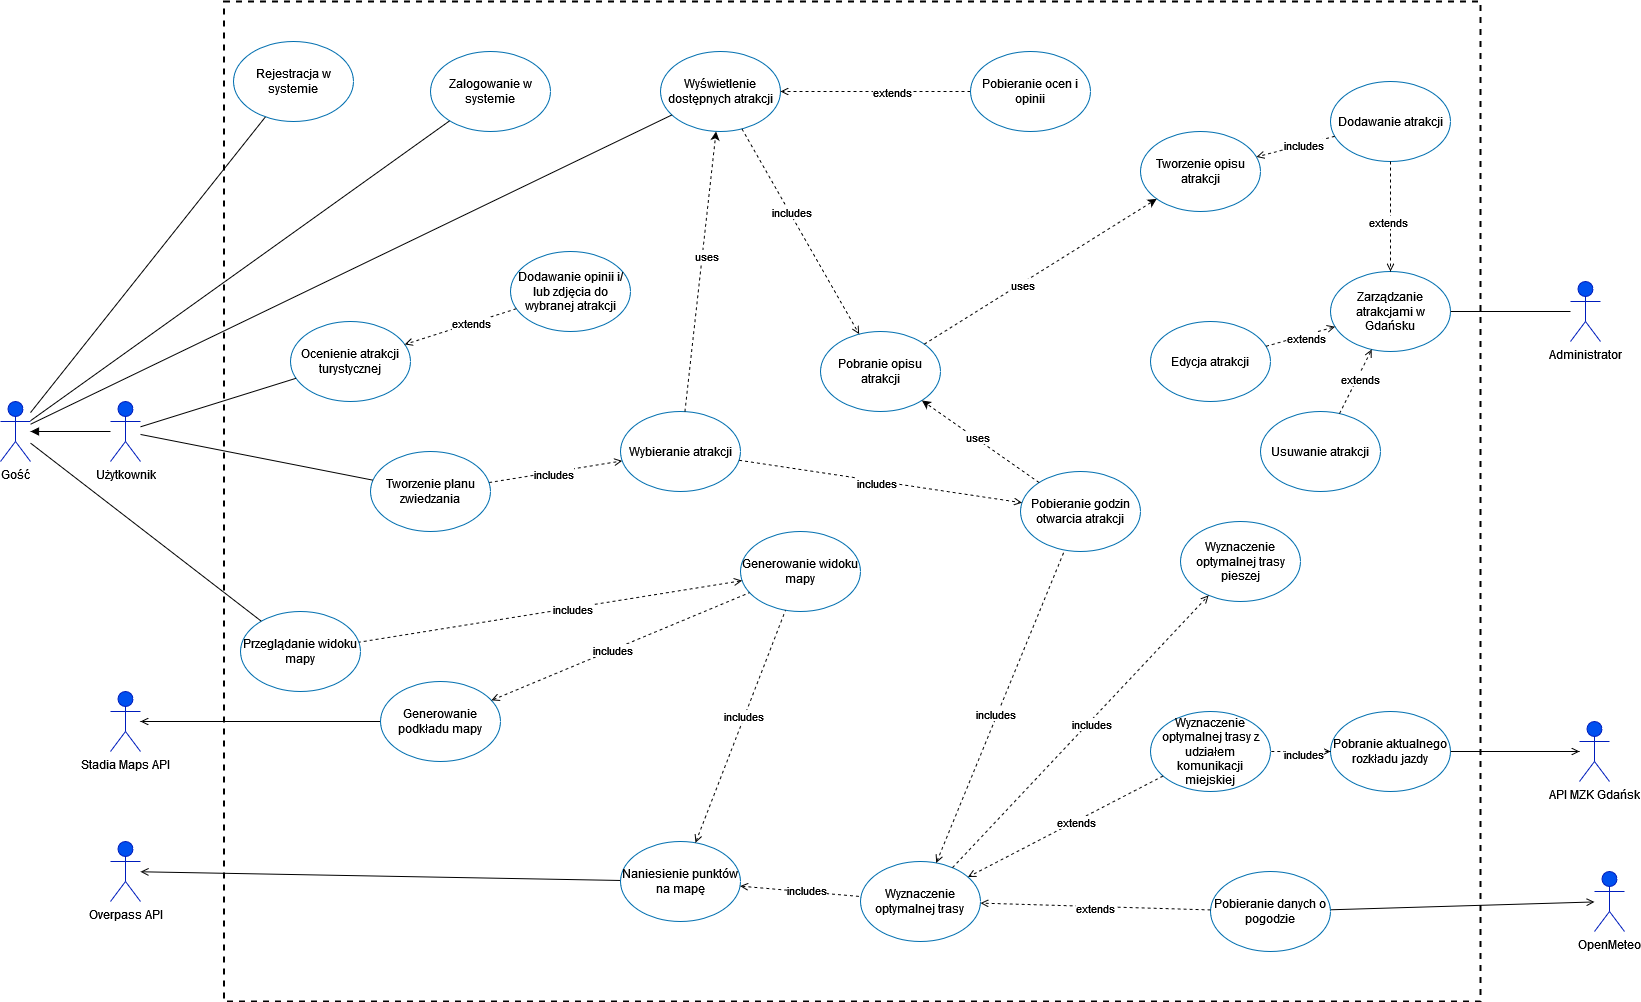
\includegraphics[width=1\textwidth]{attachments/Przypadki_Uzycia-final}
    \caption{Przypadki użycia cały projekt}
    \label{fig:przypadki-uzycia1}
    \end{figure}
Poniżej przedstawiamy przypadki użycia dla dwóch aktorów gościa oraz zalogowanego użytkownika.


    \begin{figure}[H]
        \centering
        \includegraphics[width=1\textwidth]{attachments/Użytkownik}
        \caption{Przypadki użycia aplikacji dla gościa i użytkownika}
        \label{fig:przypadki-uzycia2}
        \end{figure}

Przypadki użycia dotyczący aktorów ChatGPT oraz Administrator został przedstawiony na rysunku 4.3.

\begin{figure}[H]
    \centering
    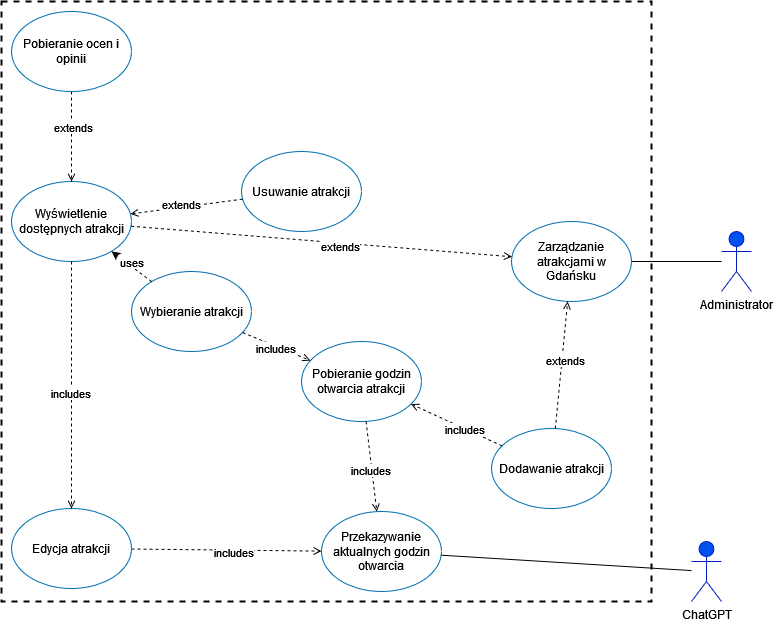
\includegraphics[width=1\textwidth]{attachments/admin}
    \caption{Przypadki użycia panel administracjny}
    \label{fig:przypadki-uzycia3}
    \end{figure}